\documentclass[a4paper,twoside]{article}


%\usepackage{ecrc}
\usepackage{epsfig}
%\usepackage{subfigure}
\usepackage{calc}
%\usepackage{amssymb}
\usepackage{amstext}
%\usepackage{amsmath}
%\usepackage{amsthm}
\usepackage{multicol}
%\usepackage{pslatex}
%\usepackage{apalike}
\usepackage{SciTePress}
\usepackage[small]{caption}
\usepackage{url}

%\subfigtopskip=0pt
%\subfigcapskip=0pt
%\subfigbottomskip=0pt

%\usepackage{doc}
%\usepackage{makeidx}
%\setlength{\textfloatsep}{10pt plus 1.0pt minus 2.0pt}

% Definitions

\def\myrelax{\textsc{Relax}}                  % TradeMarks
\def\sysml{\textsc{SysML}}
\def\UML{\textsc{Uml}}
\def\SysML{\textsc{SysML}}
\def\uml{\textsc{Uml}}
\def\kaos{\textsc{Kaos}}
\def\uppaal{\textsc{Uppaal}}

%================================================================
% remove for draft/final version
\newcommand{\final}[1]{\textbf{xxx removed for blind review purpose xxx}}
%\newcommand{\final}[1]{#1}
%================================================================

\begin{document}
\title{Early Analysis of Ambient Systems \\ \sysml{} Properties using OMEGA2-IFx}
\author{\final{\authorname{Manzoor Ahmad\sup{1}, Iulia Dragomir\sup{1}, Jean-Michel Bruel\sup{1}, Iulian Ober\sup{1} and Nicolas Belloir\sup{2}}
\affiliation{\sup{1}IRIT, Universit\'e de Toulouse, France}
\affiliation{\sup{2}LIUPPA, Universit\'e de Pau et des Pays de l'Adour, France}
\email{\{ahmad,dragomir,bruel,iulian.ober\}@irit.fr, belloir@univ-pau.fr}
}}
\keywords{Requirements, Formal Verification, Observers, \myrelax{}, Simulation}


\abstract{Formal methods provide tools to verify the consistency and correctness of a specification with respect to the desired properties of the system. This verification is important as the development of an AAL (Ambient Assisted Living) system involves different technologies (medical services, surveillance cameras, intelligent devices, etc.) requiring a strong consistency checking between models. We illustrate in this paper how we prove some of the properties of the system before the development even starts. To model the AAL system, we use the \sysml{} language. In terms of tools, we used Rational Rhapsody in combination with the OMEGA2 profile which is an executable \uml{}/\sysml{} profile used for the formal specification and validation of critical real-time systems. This profile is supported by the IFx toolset which provides mechanisms for the model simulation and properties verification of the AAL system.
}

\onecolumn \maketitle \normalsize \vfill


\section{\uppercase{Introduction}}
\label{sec:introduction}


\noindent Formal methods are intended to systemize and introduce rigor into all the phases of software development. This helps us to avoid overlooking critical issues, provides a standard means to record various assumptions and decisions, and forms a basis for consistency among related activities. By providing precise and unambiguous description mechanisms, formal methods facilitate the understanding required to coalesce the various phases of software development into a successful endeavor \cite{test1}. 

In this paper we asses the use of formal methods for the modeling and verification of Ambient Assisted Living (AAL) systems. We use the OMEGA2-IFx approach which has been applied for the verification and validation of industry-grade models \cite{test2}  providing interesting results. The OMEGA2 \UML{}/\SysML{} Profile \cite{test3} defines the semantics of \UML{}/\SysML{} elements providing the means to model coherent and unambiguous system models. In order to make the models verifiable, it presents as extension the \textit{observer} mechanism for specifying dynamic properties of models. The OMEGA2 \UML{}/\SysML{} Profile is implemented by the IFx Toolbox \cite{test4} which provides static analysis, simulation and timed-automata based model checking \cite{test5} techniques for validation.

Ambient Systems are highly adaptive. They modify their behavior at run-time in response to changing environmental conditions. For these systems, Non Functional Requirements (NFR’s) play an important role, and one has to identify as early as possible the requirements that are adaptable. The distributed nature of 
% Dynamic Adaptive Systems
these systems and changing environmental factors makes it difficult to anticipate all the explicit states in which the system will be during its lifetime. As such, they needs to be able to tolerate a range of environmental conditions and contexts, but the exact nature of these contexts remains imperfectly understood. 

For the system properties of our AAL case study, we use two types of properties: \myrelax{}-ed and Invariant. These requirements are obtained by applying a process called  \myrelax{} \cite{test6} on traditional requirements. \myrelax{}  is  a  requirement  engineering language for self-adaptive systems that incorporates uncertainty into the specification of these systems.

In \cite{test7}, we have investigated the use of goal oriented concepts in combination with \myrelax{} for modeling the requirements of ambient systems. We have found a link between \myrelax{} and \sysml{}/\kaos{} \cite{test8}, which is a goal oriented approach based on \kaos{} and which extends the \sysml{} meta-model with goal concepts. Based on that, 
we have concluded that these two approaches are complementary with each other and \myrelax{} can benefit from the ContributionNature and ContributionType concepts of \sysml{}/\kaos{}. This paper takes the reader a step forward and enriches our existing work by integrating formal methods for the verification of NFRs and specially  \myrelax{}-ed requirements.

%Typical  textual  requirements  prescribe behavior  using  a  modal  verb  such  as  SHALL  that defines  functionality  that  a  software  system  must always provide. For self adaptive systems however, environmental  uncertainty  may  mean  that  it  is  not always  possible  to  achieve  all  of  those  SHALL statements; or behavioral uncertainty may allow for trade-offs between SHALL statements to \myrelax{} non-critical  statements  in  favor  of  other,  more  critical ones.  Therefore  \myrelax{}  identifies  two  types  of requirements:  one  that  can  be  \myrelax{}ed  in  favor  of other ones called variant or \myrelax{}-ed and other that should never change called invariant.

\paragraph*{Paper structure.} This paper is organized as follows: Section~\ref{sec:r_work} presents other approaches defined for the verification of AAL models, Section~\ref{sec:tools} introduces the OMEGA2 \UML{}/\SysML{} Profile and the IFx Toolbox that are used for modeling and properties verification, Section~\ref{sec:aal_model} describes the case study: its specification, system architecture and behavior, Section~\ref{sec:properties} presents the properties, the AAL system has to satisfy, while Section~\ref{sec:results} contains the verification and simulation results, Section~\ref{sec:conclusion} concludes the paper and highlights the future work.

\section{Related work}
\label{sec:r_work}

\noindent The specification and verification of NFRs in the early stages of the AAL development cycle is a crucial issue \cite{test9}. These systems require clear and precise specifications in order to describe the system behavior and its environment. The formal specification of the system behavior supported by mathematical analysis and reasoning techniques improve their development process and enable the verification of these systems. 

In \cite{test10}, the authors present a verification approach based on MEDISTAM-RT which is a methodological framework for the design and analysis of real-time systems and timed traces to check the fulfillment of non-functional requirements. They focus on  safety and timeliness properties, to assure the correct functioning of AAL systems and to show the applicability of this methodology in the context of this kind of systems. 

In \cite{test11}, the authors introduce a profile named TURTLE (Timed \UML{} and RT-LOTOS Environment). With its formal semantics given in RT-LOTOS and its toolkit, TURTLE enables a priori detection of design errors through a combination of simulation and verification/validation techniques. By “simulation” the authors mean a partial exploration of the system state space. It is often used for debugging purposes and to quickly increase confidence in a design. For finite state space systems, exhaustive analysis is also possible. Verification relies 
on the exploration of the whole system state space in order to prove absence of deadlocks for instance and other general properties that should be satisfied by any system.

% Validation also relies on exhaustive analysis to demonstrate that a model meets specific requirements, or exhibits a certain behavior  such as the validation of a design against the requirements.

In \cite{test12}, the authors introduce \uppaal{} which is a tool box for validation (via graphical simulation) and verification (via automatic model-checking) of real-time systems. It consists of two main parts: a graphical user interface and a model-checker engine. The idea is to model a system using timed automata, simulate it and then verify properties on it. Timed automata are finite state machines with time (clocks). A system consists of a network of processes that are composed of locations. Transitions between these locations define how the system behaves. The simulation step consists of running the system interactively to check that it works as intended. Then the verifier check the reachability properties, i.e., if a certain state is reachable or not. 



%\noindent Formal methods are intended to systemize and introduce rigor into all the phases of software development. This helps us to avoid overlooking critical issues, provides a standard means to record various assumptions and decisions, and forms a basis for consistency among related activities. By providing precise and unambiguous description mechanisms, formal methods facilitate the understanding required to coalesce the various phases of software development into a successful endeavor \cite{test1}. 

%OMEGA2 \cite{test2} is an executable \uml{}/\sysml{} profile which is dedicated to the formal specification and validation of critical real-time systems. OMEGA uses the notion of \textit{observers} \cite{test2} for specifying and verifying dynamic properties of models.
%\textit{Observers} are special classes/blocks monitoring run-time state and events. They are defined by classes/blocks stereotyped with \texttt{<<observer>>}. 
%Rational Rhapsody Developer v7.5.2. \cite{test3} is used to create OMEGA2 models. 
%OMEGA2 models use a profile and a predefined library provided with the tool (OMEGA2.sbs and OMEGA2Predefined.sbs). Any other \uml{}2.2 or \sysml{}1.1 editor supporting profiling and exporting in the XMI2.0 standard compatible with Eclipse ecore can be used for OMEGA models. 

%OMEGA2 models can be simulated and properties can be verified using the IFx2 toolset \cite{test4}. 
%IFx relies on a translation of \uml{}/\sysml{} models towards a simple specification language based on an asynchronous composition of extended timed automata (IF), and on the use of simulation and verification tools available for IF. The translation takes an input model in XMI 2.0 format; it has been designed to work in conjunction with IBM Rhapsody (version 7.4 or later) but functions correctly with other XMI-compliant tools. 
%They are exported into an xmi file and then can be compiled to an executable file that can be used for simulation and verification purposes. Verification is done on the properties defined on models to check if they are satisfied or not and simulation is done for example when an error scenario is generated during a verification activity. Simulation implies to search for the error and then correct it in the corresponding model  by applying timed-automata model checking techniques \cite{test5}.

\section{\uppercase{The verification tools}}
\label{sec:tools}
\noindent In this section, we introduce the OMEGA2 Profile which we used for modeling the AAL system and its properties and the IFx toolset used for the verification and simulation of these properties. 
%\ldots

\subsection{The OMEGA2 UML/SysML Profile}

OMEGA2 is an executable \uml{}/\sysml{} profile dedicated to the formal specification and validation of critical real-time systems. It is based on a subset of \uml{} 2.2/\sysml{} 1.1 containing the main constructs for modeling system structure and class/block behavior and which provides a clear and coherent operational and timed semantics.

%\subsubsection{System structure}

The architecture of an OMEGA2 model is described in Class/Block Definition Diagrams by classes/blocks with their relationships (association, generalization and composition) and their interfaces. Each class/block defines properties and operations, as well as a state machine. The hierarchical structure of a model is defined in composite structures/Internal Block Diagrams: parts that communicate through ports and connectors. The \uml{}/\sysml{} Profile leaves open several semantic variation points for which OMEGA2 defines a set of well-formedness rules that result in a strong typing language. For further details on the rules, their rationale and formalization, the reader is referred to \cite{test13}.

%\subsubsection{Class/Block behavior}

The behavior of a system is given by the modeled state machines that use asynchronous operation calls and signal outputs for communication. The profile owns a textual action language compatible with \uml{} 2.2 action metamodel from which implements the main constructs: object creation/destruction, expression evaluation, variable assignment, signal output and control flow structuring statements.

%\subsubsection{Operational and timed semantics of OMEGA}

The operational semantics of OMEGA2 relies on an asynchronous timed execution model. Each class/block is represented by a timed input/output automata, potentially executing in parallel with other blocks and communicating via asynchronous operation calls and signals. 

The OMEGA2 Profile can model timed behavior, where the model time base can either be discrete or continuous and it is specified by the user at verification. The time model is controlled by primitives from automata with urgency \cite{test14}: clocks, time guards and transition urgency annotations. The \textit{clock} is represented by a \textit{Timer} block on which we can perform actions as: \textit{set} for setting the clock a delay and \textit{reset} to restore the clock to 0. Time guards are either described as inequalities or specified via the \textit{timeout} operation  that verifies that a certain delay has elapsed. With respect to time progress, transitions can also define a particular semantics based on their stereotype: \textit{eager} defines that time progress is disabled in a state (i.e., the actions on a transition are executed as soon as possible), \textit{delayable} means that the time progress is enabled but it is bounded by a limit and \textit{lazy} specifies that time progress is enabled and unbounded (i.e. time can progress to infinity). Based on these notions, one can also model synchronous communication in OMEGA2 model.

%\subsubsection{Observers}

For specifying and verifying dynamic properties of models, OMEGA2 uses the notion of \textit{observers}. \textit{Observers} are special classes/blocks monitoring run-time state and events. They are defined by classes/blocks stereotyped with \texttt{<<observer>>}. They may have local memory (attributes) and a state machine describes their behavior. States are classified as \texttt{<<success>>} and \texttt{<<error>>} states to express the (non)satisfaction of safety properties. The main issue in modeling observers is the choice of events which trigger their transitions, and which must include specific \uml{}/\sysml{} event types. One can observe:

\begin{itemize}
\item Events related to signal exchange: \texttt{send}, \texttt{receivesignal}, \texttt{acceptsignal}.
\item Events related to operation calls: \texttt{invoke}, \texttt{receive} (reception of call), \texttt{accept} (start of actual processing of call -- may be different from \texttt{receive}), \texttt{invokereturn} (sending of a 
return 	value), \texttt{receivereturn} (reception of the return value), \texttt{acceptreturn} (actual consumption of the return value).
\item Informal events explicitly specified by the modeller using the informal action.
\end{itemize}
The trigger of an observer transition is a \texttt{match} clause specifying the type of event (e.g., \texttt{receive}), some related information (e.g., the operation name) and observer variables that may receive related information (e.g., variables receiving the values of operation call parameters). Besides events, an observer may access any part of the state of the \uml{} model: object attributes and state, signal queues. 


\subsection{IFx Toolset}

\noindent OMEGA2 models can be simulated and properties can be verified using the IFx toolset \cite{test15}. The following terminology is used: 

\begin{description}
\item[Verification:] It designates  the  automatic  process  of  verifying  whether  an  OMEGA2  \uml{}/\sysml{} model  satisfies  (some  of)  the  properties  (i.e. \textit{observers})  defined  on  it.  The  verification  method employed in IFx is based on systematic exploration of the system state space (i.e., enumerative model checking). 
\item[Simulation:] It designates  the  interactive  execution  of  an  OMEGA2  \uml{}/\sysml{}  model.  The execution  can    be  performed  step-by-step,  random,  or  guided  by  a  simulation  scenario  (for example an error scenario generated during a verification activity). 
\end{description}

The IFx toolset relies on a translation of \uml{}/\sysml{} models towards a simple specification language based on an asynchronous composition of extended timed automata, the IF language\footnote{\url{http://www-if.imag.fr/}}. The translation takes an input model in XMI 2.0 format. 
%it has been designed to work in conjunction with IBM Rhapsody \footnote{\url{http://www.ibm.com/developerworks/rational/}} (version 7.4 or later) but functions correctly with other XMI-compliant tools. 
The compiler verifies the set of well-formedness rules imposed by the profile and generates an IF model that can be further reduced by static analysis techniques. This model is subject to verification that either validates the model with respect to its properties or produces a list of error scenarios that can be further debugged using the simulator. The overall workflow  of IFx Toolset is shown in Fig.~\ref{fig:flow} \cite{test16}.

\begin{figure}[!htb]
%\begin{figure*}[!h]
  \centering
  {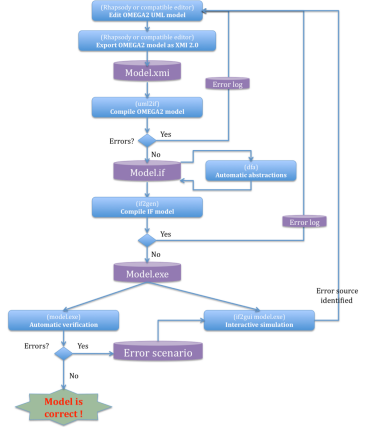
\epsfig{file =Workflow, width = 8cm}}
  \caption{IFx Workflow}
  \label{fig:flow}
%\end{figure*}
\end{figure}
 

%\vfill

\section{\uppercase{Modeling the AAL system with OMEGA2 Profile}}
\label{sec:aal_model}
\noindent In this section, we explore the AAL system specification, the system architecture showing its structural and behavioral diagrams i.e. its block definition diagram, internal block diagrams and state machine diagrams.

\subsection{System Specification}
Here is an excerpt of the AAL case study \cite{test6}: \textit{Mary is a widow. She is 65 years old, overweight and has high blood pressure and cholesterol levels. Following her doctor’s instructions, she is considering to loose weight. The doctor has recommended a hypo caloric diet with low levels of salt. She lives by herself in an AAL house}.
First, we start by taking into account the structural part of the AAL system. We consider those parts that are concerned with the daily calories intake of the \texttt{Patient} in the AAL house. The AAL system is composed of \texttt{Fridge} and \texttt{Patient}. We would like to model these parts and the interaction that takes place between them. The \texttt{Fridge} partially contributes to the minimum liquid intake of the \texttt{Patient}; it also looks at the calories consumption of the \texttt{Patient} as he/she does not need to exceed it after a certain threshold. 

\subsection{System Architecture}
Fig.~\ref{fig:mainibd} shows the main internal block diagram. The important parts of the AAL system are \texttt{Patient} and \texttt{Fridge}. A \texttt{Fridge} in turn is composed of \texttt{Food}, \texttt{Display}, \texttt{Alarm} and \texttt{Controller} blocks. The \texttt{Food} block contains information about the food items in the \texttt{Fridge}, the calories contained by each item, the total number of calories the \texttt{Patient} has accumulated and the calories threshold that should not be surpassed. The fridge \texttt{Display} is used to show the amount of calories consumed by the \texttt{Patient}. The \texttt{Alarm} is activated in case the \texttt{Patient}'s calories level surpasses a certain threshold. The \texttt{Controller} transfer the information from the \texttt{Patient} to the concerning elements and back to the environment. 

The communication between different blocks takes place through ports. A  port  bears  a  type.  In  OMEGA2,  the  type  of  a  port  must  be  an  Interface. The type specifies the set of requests (operation calls and/or signals) that  are transferred between parts (components) by means of ports and connectors. In Fig.~\ref{fig:mainibd}, the \texttt{Patient} block has a standard port named \texttt{pToFridge}. This port has a contract named \texttt{Patient2Fridge} and is acting as a provided interface of the \texttt{Patient} block. The interface \texttt{Patient2Fridge} defines an operation \texttt{eat(int item, int quantity)}. This interface is then used as a type of \texttt{pToFridge} port. At the same time the \texttt{Patient} block has a required interface named \texttt{pFromPatient}. For the full system architecture, the reader is referred to \cite{test17}.

Rational Rhapsody Developer v7.5.2\footnote{http://www.ibm.com/developerworks/rational/} is used to create OMEGA2 models. OMEGA2 models use a profile and a predefined library provided with the tool (OMEGA2.sbs and OMEGA2Predefined.sbs). Any other \uml{}2.2 or \sysml{}1.1 editor supporting profiling and exporting in the XMI2.0 standard compatible with Eclipse ecore can be used for OMEGA2 models.

\begin{figure}[!h]
  \centering
  {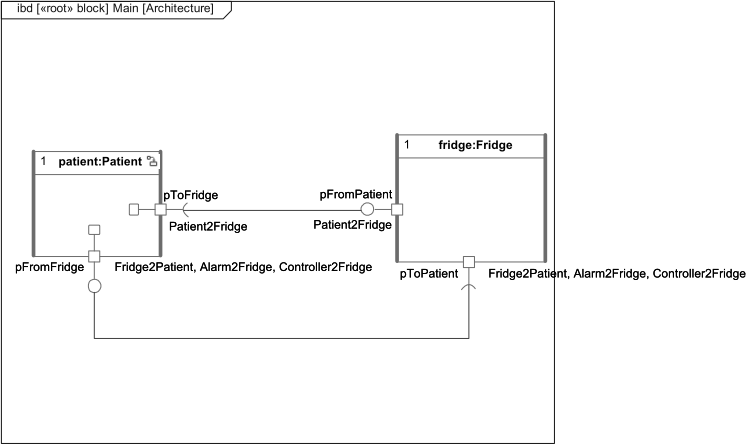
\epsfig{file =MainIBD, width = 8cm}}
  \caption{Main Internal Block Diagram}
  \label{fig:mainibd}
 \end{figure}
 
%The important part of the AAL system is the intelligent \texttt{Fridge}. 
The \texttt{Fridge} interacts with the AAL system. Fig.~\ref{fig:fridgeibd} shows the internal block diagram for the \texttt{Fridge} block. Each of the four blocks behaviors is modeled in a separate state machine diagram.

\begin{figure}[!h]
  \centering
  {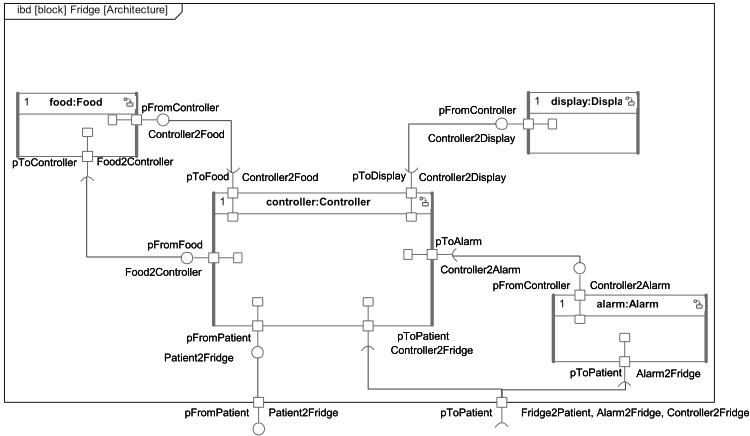
\epsfig{file =FridgeIBD, width = 8cm}}
  \caption{Fridge Internal Block Diagram}
  \label{fig:fridgeibd}
 \end{figure}
 
Fig.~\ref{fig:patientstm} shows the state machine diagram for the \texttt{Patient} block. Here the exchange of information between \texttt{Patient} and \texttt{Fridge} takes place. We identify the number and quantity of each item present in the \texttt{Fridge}. If a certain product still present in the \texttt{Fridge} is chosen by the \texttt{Patient} then the information is  communicated with the \texttt{Fridge}.  Otherwise the \texttt{Fridge} is empty and the \texttt{Patient} will wait to be refilled. Also, if the \texttt{Alarm} of the \texttt{Fridge} is raised due to  high intake of calories, the \texttt{Patient} stops eating and waits for the system to be unblocked.
 
\begin{figure}[!h]
  \centering
  {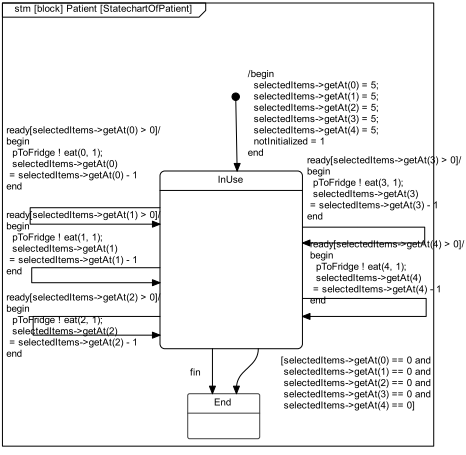
\epsfig{file =PatientSTM, width = 8cm}}
  \caption{Patient State Machine Diagram}
  \label{fig:patientstm}
 \end{figure}
 
The \texttt{Food} block models the knowledge of the \texttt{Fridge} about what it contains. We define the number of items and the amount of calories associated with each item present in the \texttt{Fridge}. We then calculate the total number of calories accumulated by the \texttt{Patient}. If the total number of calories is greater or equal to the maximum calories allowed for the \texttt{Patient}, then a message is sent and the alarm is raised or if the total number of calories is greater than the maximum calories allowed minus 500, then the \texttt{Patient} is warned with a message that the calories level is approaching the maximum amount of calories allowed. 

%Fig.~\ref{fig:foodstm} shows the state machine diagram for the Food block.

%\begin{figure}[!h]
%  \centering
%  {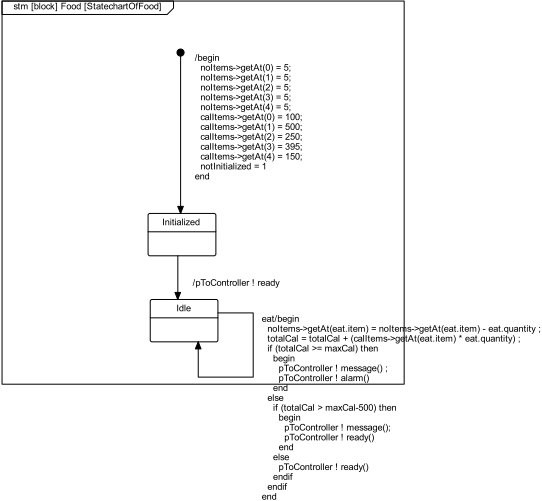
\epsfig{file =FoodSTM, width = 8cm}}
%  \caption{Food State Machine Diagram}
%  \label{fig:foodstm}
% \end{figure}

\section{\uppercase{Properties Verification of AAL system}}
\label{sec:properties}
\noindent The properties of AAL system that we modeled and verified are obtained after \myrelax{} process is applied on its traditional requirements. \myrelax{}  is  a  requirement  engineering language for self-adaptive systems that incorporates uncertainty into the specification of these systems. Typical  textual  requirements  prescribe behavior  using  a  modal  verb  such  as  SHALL  that defines  functionality  that  a  software  system  must always provide. For self adaptive systems such as AAL, however, environmental  uncertainty  may  mean  that  it  is  not always  possible  to  achieve  all  of  those  SHALL statements; or behavioral uncertainty may allow for trade-offs between SHALL statements to \myrelax{} non-critical  statements  in  favor  of  other,  more  critical ones.  Therefore,  \myrelax{} identifies two types of requirements: one that can be \myrelax{}-ed in favor of other ones called variant or \myrelax{}-ed and other that should never change called invariant.
Below are the properties to be verified. 

\subsection{Traditional/\myrelax{}-ed Requirement}

\noindent We have studied two \myrelax{}-ed requirements:
\begin{itemize}
\item The fridge shall detect and communicate with food packages
\end{itemize}

\myrelax{}-ed version of this requirement is as follows:

\begin{itemize}
\item Property 1 : The fridge SHALL detect and communicate information with AS MANY food packages AS POSSIBLE
\end{itemize}

Below are the uncertainty factors associated with the given \myrelax{}-ed requirement.

\begin{description}
\item[ENV:] Food locations, foot item information (type, calories), food state (spoiled and unspoiled)
\item[MON:] RFID readers, Cameras, Weight sensors
\item[REL:] RFID tags provide food locations and food information; Cameras provide food locations (Cameras provide images that can be analyzed to estimate food locations), Weight sensors provide food information (whether eaten or not)
\end{description}

\begin{figure}[!h]
  \centering
  {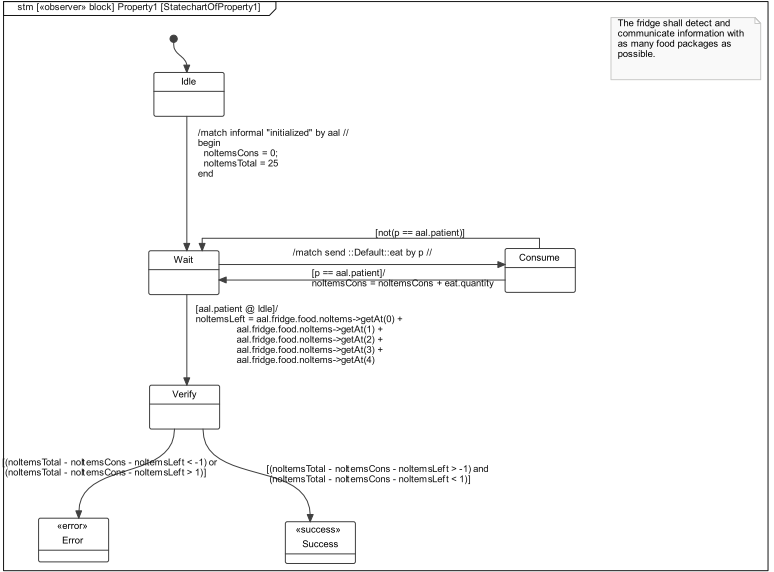
\epsfig{file =Property1STM, width = 7cm}}
  \caption{Property1 State Machine Diagram}
  \label{fig:property1stm}
 \end{figure}
 
The satisfaction of this requirement contributes to the balanced diet of the \texttt{Patient}. We would like to verify this property as it is important for the AAL system to know about as many food items as possible present in the \texttt{Fridge}. Fig.~\ref{fig:property1stm} shows the state machine diagram of the Property 1. In this property, we identify the number of items consumed by the \texttt{Patient} and the total number of items in the \texttt{Fridge}. First of all, we verify the identity of the \texttt{Patient}, if the person is identified as the \texttt{Patient}, then we calculate the number of items consumed. We then calculate the number of items left in the \texttt{Fridge} which is equal to the sum of all the items present in the \texttt{Fridge}. Then in the last step, we calculate if ((total number of items - number of items consumed - number of items left) \textgreater -1) and ((total number of items - number of items consumed - number of items left) \textless 1),
it means that we have reached the \texttt{<<success>>} state by having information about all the items present in the \texttt{Fridge}, i.e. it should be 0 (which means that there is no information loss). Inversely, if it is less than -1 and greater than 1, then it means that we are missing information about some of the items present in the \texttt{Fridge} and the \textit{observer} passes into the \texttt{<<error>>} state.

% the total number of items minus the number of items consumed minus the number of items left is less than -1 or the total number of items minus the number of items consumed minus the number of items left is greater than 1, 

\subsection{Invariant Requirement}
\noindent We have taken two examples of invariants:

\begin{itemize}
\item Property 2 : The alarm SHALL be raised instantaneously if the total number of calories surpasses the maximum calories allowed for the patient 
\end{itemize}

\begin{figure}[!h]
  \centering
  {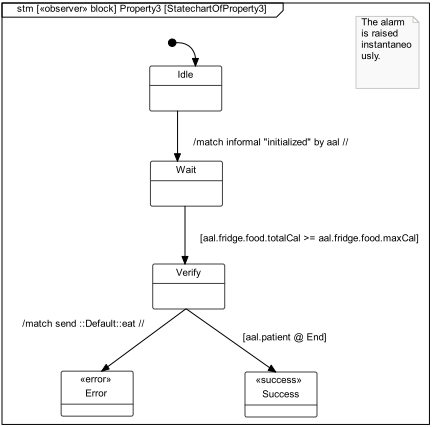
\epsfig{file =Property3STM, width = 8cm}}
  \caption{Property2 State Machine Diagram}
  \label{fig:property3stm}
 \end{figure}
 
  
This property ensures that the \texttt{Patient} should stop eating when the total number of calories surpasses the maximum calories allowed and that the Alarm should be raised. Fig.~\ref{fig:property3stm} shows the state machine diagram of the property 2. This requirement implies that the Alarm shall be immediately raised as soon as the total number of calories equals or surpasses the maximum calories allowed for the \texttt{Patient}. If it happens then the \texttt{Patient} should stop eating.  

\section{Verification Results}
\label{sec:results}
%\subsection{Verification Results}
\noindent Until now, we have modeled the AAL system and the properties to be verified on the model. It is now time to verify these properties and in case if there is error during its verification, simulate it to find the error and then correct it in the model. Fig.~\ref{fig:xmi2if} shows the snapshot of the compilation of the AAL model named AAL2. The AAL2 model is first exported into \texttt{AAL2.xmi} and then using the IFx toolset the \texttt{AAL2.xmi} is compiled into \texttt{AAL2.if}.

\begin{figure}[!h]
  \centering
  {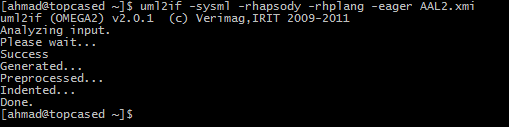
\epsfig{file =Xmi2If, width = 8cm}}
  \caption{XMI to IF Compilation}
  \label{fig:xmi2if}
 \end{figure}
  
%\begin{figure}[!h]
%  \centering
%  {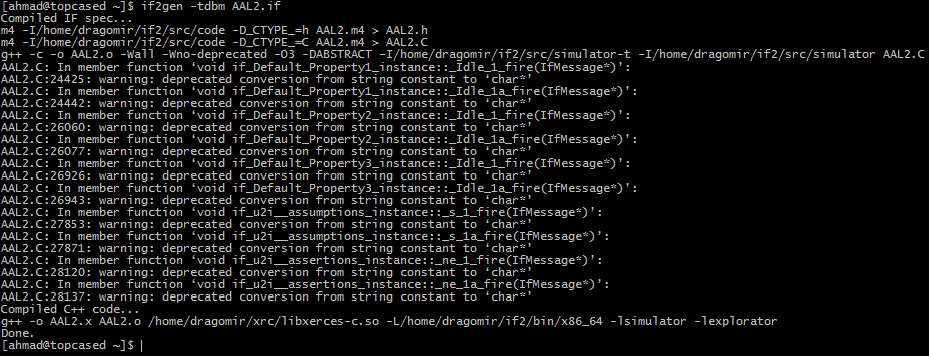
\epsfig{file =If2Exe, width = 8cm}}
%  \caption{IF to Executable file Compilation}
%  \label{fig:if2exe}
% \end{figure}
 
%Fig.~\ref{fig:if2exe} shows the snapshot of the compilation of AAL2.if into an executable file i.e. AAL2.x. 
The AAL2.if is then compiled into an executable file i.e. AAL2.x.
For the properties verification part, we run the model-checker with the following options:
\texttt{AAL2.x -dfs -po -me -ce –ln}

While verifying the AAL model, the model-checker has found several error scenarios. 
%as can be seen in Fig.~\ref{fig:errorstate}.
Any of the error scenario can then be loaded through the interactive simulation interface of the IFx toolset to trace back the error in the model and then correct it. 
%
%\begin{figure}[!h]
%  \centering
%  {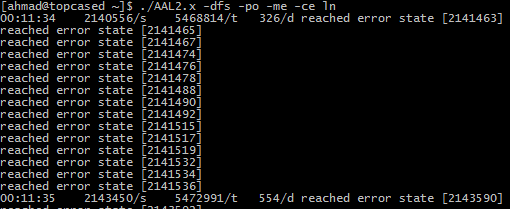
\epsfig{file =ErrorState, width = 8cm}}
% \caption{Model Checker results in Error Scenarios}
% \label{fig:errorstate}
%\end{figure}
%
\begin{figure}[!h]
  \centering
  {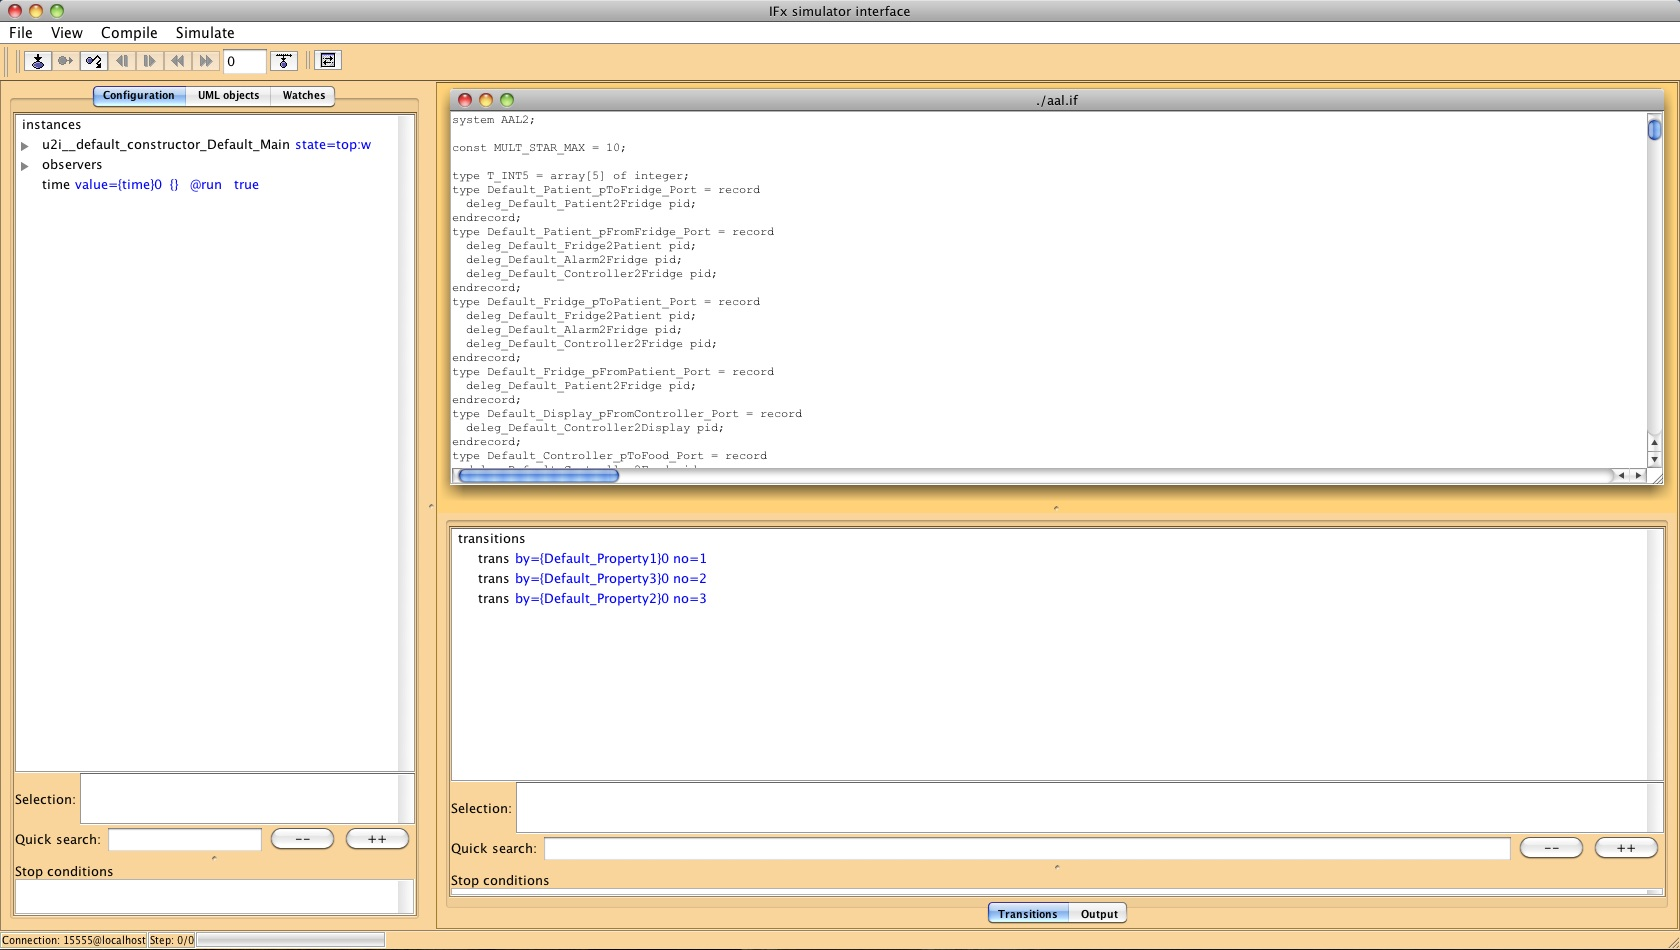
\epsfig{file =InitialSimulationInterface, width = 8cm}}
  \caption{Initial Simulation Interface}
  \label{fig:initialsimulationinterface}
 \end{figure}
%
In order to  debug  a model, firstly we import it into the simulator as shown in Fig.~\ref{fig:initialsimulationinterface}. We check the states of the \textit{observers} in order to identify which property has not been satisfied. One can observe in Fig.~\ref{fig:errorstatefoodobserver} that Property 2 fails. While checking the state of the entire system for this property, we discover that the error state contained the maximum allowed number of calories for the total number of calories consumed and subsequently eat requests sent by the \texttt{Patient}. This implies that the Alarm function of the intelligent \texttt{Fridge} doesn't function properly. The Alarm function of the \texttt{Fridge} is strictly linked to its Food process and the Alarm is raised only if the total number of consumed calories is strictly superior than the maximum allowed; condition which doesn't satisfy the request that the Alarm is raised as soon as possible. The correction consists in raising the Alarm in case the total number of consumed calories is equal to the maximum allowed threshold. Once this error is corrected the verification succeeds.

%One can observe in the state machine of the Food block (Fig.~\ref{fig:foodstm}) 

\begin{figure}[!h]
  \centering
  {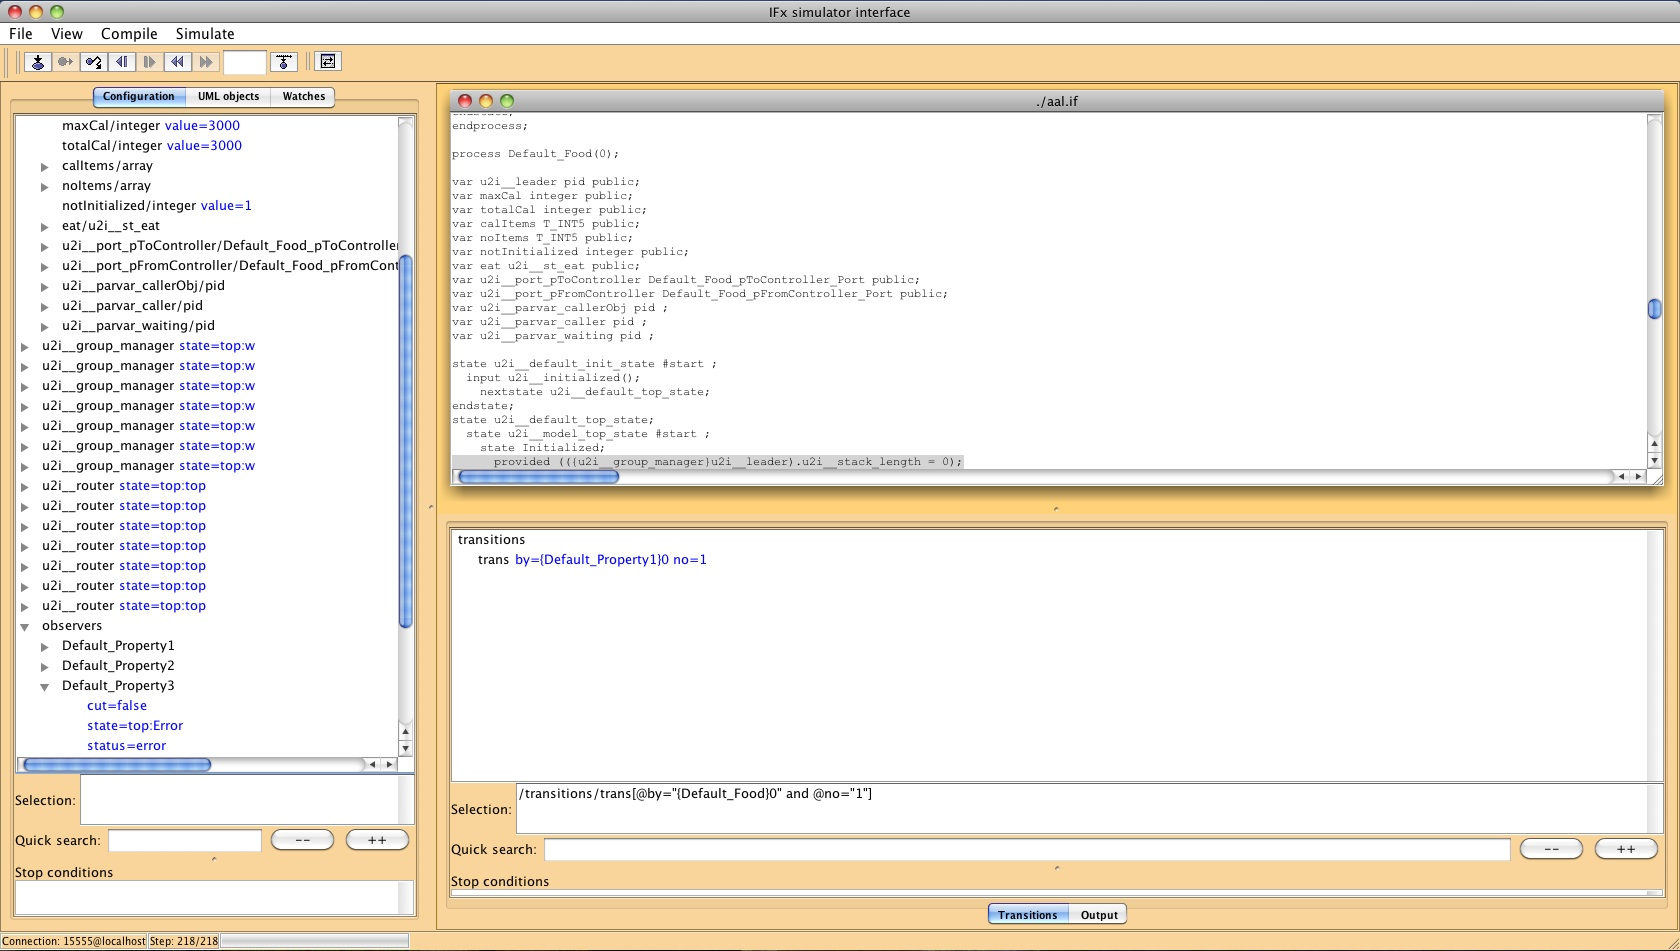
\epsfig{file =ErrorStateFoodObserver, width = 8cm}}
  \caption{Error State Food Observer Simulation Interface}
  \label{fig:errorstatefoodobserver}
 \end{figure}

\begin{figure}[!h]
  \centering
  {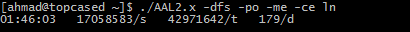
\epsfig{file =VerificationOk, width = 8cm}}
  \caption{Model checking successful}
  \label{fig:verificationok}
 \end{figure} 

Fig.~\ref{fig:verificationok} shows the result of the model-checker on the correct model.

\section{{Conclusion}
\label{sec:conclusion}}
We have modeled the structural and behavioral parts of an AAL (Ambient Assisted Living) system. The modeling is done using Rational Rhapsody 7.5.2  with OMEGA2 profile which is used for specification and verification of dynamic properties of models through \textit{observers}. For the verification and simulation part, we have used IFx which is a toolset used for the simulation of OMEGA2 models and the verification of properties defined on these models. We have verified two properties of the AAL system using the IFx toolset. At first, the verification results in errors which can then be simulated through the interactive simulation interface of the IFx toolset in order to identify the source of the error and then subsequently correct it in the model, after correcting the error in the model, the verification results in the fulfilment of all the two properties. 

The future work is centred around the use of formal methods in the context of our integrated approach \cite{test18}. This work motivated us to take benefit from the OMEGA2/IFx. In our integrated approach, we are interested in \myrelax{} requirement which we obtain by using the \myrelax{} process. We then refine the \myrelax{} requirement with the \texttt{ContributionType} and \texttt{ContributionNature} of \sysml{}/\kaos{} which is a \sysml{} profile with the goal concepts integrated into it, the reader is referred to \cite{test7} for an insight on our work on \myrelax{} and \sysml{}/\kaos{}. The \myrelax{} requirement is then verified by a test case that can be refined by observer. The observer is then allocated to a state machine diagram. This whole sequence of steps constitute our process.

%The application of OMEGA2 profile to models is straight forward in that one only needs to add the predefined library provided with the tool (OMEGA2.sbs and OMEGA2Predefined.sbs) into the model. After the creation of OMEGA2 models, export to an xmi file is simply done through the Rational Rhapsody v7.5.2 menu. The choice of the version of Rational Rhapsody is very important as OMEGA2/IFx is not compliant with the new versions of Rational Rhapsody. Another important point to mention is the time the IFx toolset takes for the verification of properties as it depends on the number of items present in the \texttt{Fridge} i.e. in our case study, we have five items in the \texttt{Fridge} and the model checker took considerable amount of time to check all the states of the system. 

%\bibliographystyle{apalike}
%{\small
%\bibliography{example}}

\begin{thebibliography}{1}

\bibitem{test1} 
\url{http://www-2.cs.cmu.edu/~svc/}

\bibitem{test2}
\final{Iulia Dragomir, Iulian Ober and David Lesens. A Case Study in Formal System Engineering with SysML, ICECCS 2012,Pages: 189 - 198.}

\bibitem{test3} \final{Iulian Ober and Iulia Dragomir. OMEGA2: A new version of the profile and the tools, ICECCS 2010,
DOI 10.1109/ICECCS.2010.59.}

\bibitem{test4}  \final{Iulian Ober, Susanne Graf and Ileana Ober. Validating timed \uml{} models by simulation and verification, International Journal on Software Tools for Technology (2006) 8(2): 128–145}

\bibitem{test5}E. M. Clarke, O. Grumberg, and D. A. Peled, Model Checking. MIT Press, 1999.

\bibitem{test6} \final{Jon Whittle, Pete Sawyer, Nelly Bencomo, Betty H.C. Cheng, and Jean-Michel Bruel. \myrelax{} : Incorporating Uncertainty into the Specification of Self-Adaptive systems,RE Conference 2009, Pages: 79-88.}

\bibitem{test7} \final{Manzoor Ahmad, Jean Michel Bruel, R\'egine Laleau and Christophe Gnaho. Using RELAX, SysML and KAOS for Ambient Systems Requirements Modeling, Procedia Computer Science Volume 10, 2012, Pages 474–481.}

\bibitem{test8} Christophe Gnaho, Farida Semmak. Une extension \sysml{} pour l'ing\'enierie des exigences non-fonctionnelles orient\'ee but. Revue Ing\'enierie des Syst\`emes d'Information, Vol 16/1, 23 pages, 2011.

\bibitem{test9} Kawtar Benghazi, Mar\'ia Visitaci\'on Hurtado, Mar\'ia Luisa Rodr\'iguez, Manuel Noguera. Applying Formal Verification Techniques to Ambient Assisted Living Systems, OTM 2009 Workshops, pp 381-390.

\bibitem{test10} J\"urgen Nehmer, Martin Becker, Arthur Karshmer and Rosemarie Lamm. Living assistance systems: an ambient intelligence approach, ICSE '06, Pages 43-50. 

%Benghazi, K.: MEDISTAM–RT: Metodolog´ıa de dise˜no y an´alisis de sistemas de tiempo real. PhD Thesis, University of Granada, Spain (2009)

\bibitem{test11} Ludovic Apvrille, Pierre de Saqui-Sannes, Ferhat Khendek. TURTLE-P: a \UML{} profile for the formal validation of critical and distributed systems, Software and System Modeling 5(4): 449-466 (2006).

\bibitem{test12} \url{http://www.it.uu.se/research/group/darts}
%/uppaal/
%small_tutorial.pdf

\bibitem{test13}
\final{I.~Ober and I.~Dragomir, ``{Unambiguous \UML{} Composite Structures: The OMEGA2 Experience},'' in \emph{SOFSEM 2011: Theory and Practice of Computer Science}, \hskip 1em plus 0.5em minus 0.4em\relax Springer, 2011, vol. 6543, pp. 418--430.}


\bibitem{test14}
S.~Bornot and J.~Sifakis, ``{An algebraic framework for urgency},'' \emph{Information and Computation}, vol. 163, 2000.

\bibitem{test15}
\final{M.~Bozga, S.~Graf, I.~Ober, I.~Ober, and J.~Sifakis, ``{The IF Toolset},'' in \emph{Formal Methods for the Design of Real-Time Systems}, \hskip 1em plus 0.5em minus 0.4em\relax Springer, 2004, vol. 3185, pp. 131--132.}

\bibitem{test16} OMEGA2-IFx for \uml{}/\sysml{} v2.0 Profile and Toolset, User Manual Document v1.1

\bibitem{test17} \final{Manzoor Ahmad, Iulia Dragomir. AAL System Properties Modeling and Verification Using OMEGA2/IFx, Internal Report, Universit\'e de Toulouse.}

%\bibitem{test18}  IBM, “Rational Rhapsody v7.5. reference manuals.” Available via \url{http://www.ibm.com/developerworks/rational/}.

\bibitem{test18} \final{Jean-Michel Bruel, Nicolas Belloir and Manzoor Ahmad. SPAS: un profile \sysml{} pour les syst\`emes auto-adaptatifs, CNRIUT, Lille June 2009.}





\end{thebibliography}

%\section*{\uppercase{Appendix}}
%
%\noindent If any, the appendix should appear directly after the
%references without numbering, and not on a new page. To do so please use the %following command:
%\textit{$\backslash$section*\{APPENDIX\}}
\vfill
\end{document}

